 \documentclass[12pt]{article}
 
\setlength{\parindent}{4em}
\usepackage{url}

\usepackage{bm,nicefrac}
\usepackage{amsmath,amssymb,amsthm,amsfonts}
\usepackage{wasysym}
\usepackage{graphicx}
\graphicspath{{figures/}}
\frenchspacing
\usepackage{xcolor}
\usepackage{relsize}
\usepackage{stackengine}
\newcounter{subfigure}
\usepackage[colorlinks]{hyperref}
\usepackage{multirow}
\usepackage{algorithm}
\usepackage{algpseudocode}
\usepackage{tcolorbox}
\usepackage{calc}
\usepackage{mathtools}  
\usepackage{geometry}
\usepackage{appendix}

\usepackage{listings}
\definecolor{codegreen}{rgb}{0,0.6,0}
\definecolor{codegray}{rgb}{0.5,0.5,0.5}
\definecolor{codepurple}{rgb}{0.58,0,0.82}
\definecolor{backcolour}{rgb}{0.95,0.95,0.92}

\lstdefinestyle{mystyle}{
    backgroundcolor=\color{backcolour},   
    commentstyle=\color{codegreen},
    keywordstyle=\color{magenta},
    numberstyle=\tiny\color{codegray},
    stringstyle=\color{codepurple},
    basicstyle=\ttfamily\footnotesize,
    breakatwhitespace=false,         
    breaklines=true,                 
    captionpos=b,                    
    keepspaces=true,                 
    numbers=left,                    
    numbersep=5pt,                  
    showspaces=false,                
    showstringspaces=false,
    showtabs=false,                  
    tabsize=2
}

\lstset{style=mystyle}


\geometry{top = 1in, bottom = 1in, left = 1in, right = 1in}


\begin{document}
 
% --------------------------------------------------------------
%                         Start here
% --------------------------------------------------------------
 
\title{A  Brief Report on Neural Networks with Pytorch Implementation}
\author{Erdi KARA}
\date{}
\maketitle
 
\section*{Introduction}

	
	In this small course report, we will try to explain the underlying ideas of neural networks. We first briefly introduce the mathematics behind it and then give a quick overview on regularization techniques. Lastly, based on these tools, we will create an algorithm for a basic image classification problem using Pytorch. \cite{torch}



\section{ Feedforward Neural Networks}
\subsection{Preliminary Concepts}
\label{PC}

Deep learning can be considered as a subclass of machine learning that utilize multiple-layer architecture to extract information from a given data. Each layer consist of units, called \textit{neurons}, which is a numerical representation of the processed information. Each neuron in the architecture has two typical parameters (possibly other parameters as well), \textit{a weight} and \textit{a bias}. A neural network architecture is composed of an \textit{ input layer, hidden layer(s) } an \textit{output layer}. Each hidden layer has a certain level of connection with the previous and the next layer.  We define the \textit{depth} of a network  as the number of layers except the first one while the \textit{width} is the the maximum number of neurons in a layer. A network with depth 4 and width 8 can be seen in Figure \ref{fig:nnpic} where weights and biases are displayed in matrix form which we will see later.


\begin{figure}[H]
  \centering
  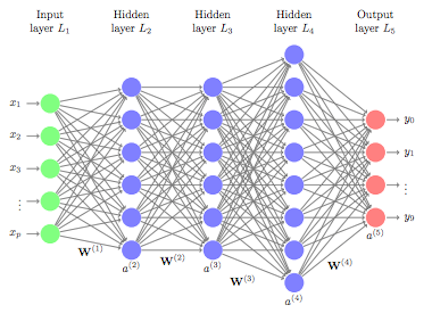
\includegraphics[width=0.75\textwidth]{network.png}
  \label{fig:nnpic}
\end{figure}


Input layer is used to hold the row input data. We then pass the data to the hidden layers which process this data using weights and biases of the neurons belonging to the layer. Passing the information from one layer to another is called a \textit{forward pass}. By this way, information flows through the hidden layers until the output layer. After the forward pass is completed, we compute the loss of the algorithm against a known true value using a \textit{cost function}. In other words, we measure the quality of the prediction. We then use this information to update the weights and biases of the layers starting from the last one to the first. This backward-updating process is called \textit{back propagation}. 
We process the entire data by forward-passing and back propagating. One such complete cycle is called an \textit{epoch}. We repeat the same process for several epochs to improve the quality of the prediction. The main goal is to update the weights and biases (possibly other parameters as well) to minimize the cost function in each epoch so that we can obtain more accurate predictions.

Deep neural network (DNN) can be regarded as a collective name of all similar methods. The network above is called the feed forward (sometimes multilayer perceptrons) because the output is not fed back to the system. Neural networks having this property are called recurrent neural networks(RNN). Another type of neural network is the convolution neural networks (CNN) which we will discuss in Section \ref{CNN}. In this report, we primarily focus on feed forward and convolution networks. However, fundamental principles we will discuss in the next section is applicable in a broad range of neural network models.   
 


\subsection{Mathematical Foundations}
\label{MF}
\subsubsection{Motivation}
\label{mt}
In mathematical terms, a feed forward neural network defines an approximation scheme  \bm{$y=F(x;\theta)$}  to approximate a function $y=f(x)$. The network optimizes or \textit{learns} the parameter family \bm{$\theta$} to find the best approximation to the function $f(x)$. We can start with an illustrative example. Consider the sample data in table below. 
%It is spesifically generated so that $7X1+2X2=Y$. 

\begin{center}
\begin{tabular}{ |c|c|c| } 
\hline
$X_1$ & $X_2$ & Y \\ 
\hline
3&	3&  27 \\
8&	6&	68 \\
8&	1&	58 \\
3&	4&	29 \\
1&	6&	19 \\
4&	9&	46 \\
\hline
\end{tabular}
\end{center}

Our task is to build a \textit{network(model,arhitecture,..)} to predict the output $Y$ given $X_1$ and $X_2$. Consider the following network with 2 input neurons 
and a single output. Two neurons represent two real input values $x_1,x_2$  and $\hat{y}$ is the predicted output in each row. As a convention, weights and bias belong to the next layer. 
\begin{figure}[h]
  \centering
  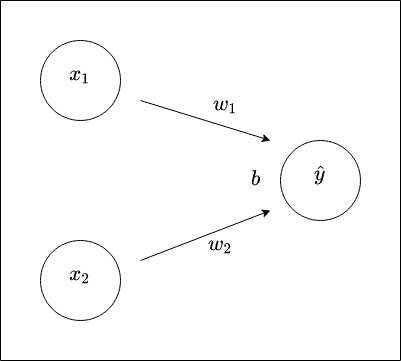
\includegraphics[width=0.25\textwidth]{2x1.png}
  \caption{A neural network with two layers; two inpus in the first layer no hidden layer and one output in the output layer}
\end{figure} 

\noindent Let's start with  a \textit{linear model}. In other words,
\begin{equation}
\label{eq:model}
\hat{y}=w_{1}x_{1}+w_{2}x_{2}+b
\end{equation}
for the weights $w_1,w_2$ and the bias $b$. In machine learning terminology, we call them \textit{learnable parameters}. To measure the error between the predicted value $\hat{y}$ and the real ouput $y$, we need a \textit{cost function}. The easiest way is to consider the mean-square cost function 

%
% $$C(\hat{y})=\dfrac{1}{N}\sum_{i=1}^{N}\Big(\hat{y}_i -y_i\Big)^2 =
% \dfrac{1}{N}\sum_{i=1}^{N}\Big(w_{1}x_{1}^{(i)}+w_{2}x_{2}^{(i)}+b -y_i\Big)^2 $$
%
%Using chain rule, we can see that $$\dfrac{\partial C}{\partial w} = \dfrac{1}{N}\sum_{i=1}^{N}2\Big(y(x_i)-y_i\Big)x_i$$, $$ \dfrac{\partial C}{\partial b} = \dfrac{1}{N}\sum_{i=1}^{N}2\Big(y(x_i)-y_i\Big)1$$

\begin{equation}
\label{eq:cost}
C(\hat{y})=\dfrac{1}{N}\sum_{i=1}^{N}\Big(\hat{y}_i -y_i\Big)^2 =
 \dfrac{1}{N}\sum_{i=1}^{N}\Big(w_{1}x_{1}^{(i)}+w_{2}x_{2}^{(i)}+b -y_i\Big)^2
\end{equation}
\noindent where, $\left(x_1^{(i)},x_2^{(i)}\right)$ are the input values in the $i^{\text{th}}$ row. Notice that the cost function is over all predictions. With these ingredients, the problem statement reads 
\begin{center}
\textit{Find $w_1,w_2,b$ such that $C(\hat{y})$ is minimized.}
\end{center} 
Thus, the core idea in a neural network is to find the optimal values of learnable parameters to minimize the cost function so that $\hat{y}_i \approx y_i$ for each data points. The most common method to tackle this problem is the \textit{gradient decent} algorithm.  

It is very well known that the maximum rate of decrease of a differentiable function occurs in the direction of the negative gradient. The cost function we define is an \textit{implicit function} of learnable parameters. 
The idea is to evaluate the gradients of the cost function with respect to the learnable parameters and take repeated steps in the direction of the negative gradient, which will lead to the local minimum(ideally the global minimum) of the cost function. 
The step size taken is called the \textit{learning rate}. This quantity measures how fast we update the learnable parameters. One step gradient decent can be summarized as follows where we set the learning rate $r=0.01$

\begin{enumerate}
\item Initilize the weights and biases(only once)
$w_1=5,w_2=2,b=3$
\item Forward Pass
\begin{enumerate}
\item Feed the data

inputs: $\left(x_1^{(i)},x_2^{(i)}\right)$ and outputs: $y_i$ for $i=1,2,..N$
\item Get the predictions $\hat{y}_i$

$\hat{y}_i=w_{1}x_{1}^{(i)}+w_{2}x_{2}^{(i)}+b = 5\cdot2+2\cdot8+3=29$
\item Evaluate the loss $C(\hat{y})$

$C(\hat{y})=(\hat{y}-y)^2 = (29-(-1))^2=900$
\end{enumerate}
\item Back Propogation
\begin{enumerate}
\item Evaluate the gradients

$\dfrac{\partial C}{\partial w_{1}} = \dfrac{\partial C}{\partial \hat{y}} \dfrac{\partial \hat{y}}{\partial w_1}=2(\hat{y}-y)x_1 = 2(29-(-1))2=120 $ 

$\dfrac{\partial C}{\partial w_{2}} = \dfrac{\partial C}{\partial \hat{y}} \dfrac{\partial \hat{y}}{\partial w_2}=2(\hat{y}-y)x_2 = 2(29-(-1))8=480 $

$\dfrac{\partial C}{\partial b} = \dfrac{\partial C}{\partial \hat{y}} \dfrac{\partial \hat{y}}{\partial b}=2(\hat{y}-y)1 = 2(29-(-1))1=60 $
\item Update the weights(gradient decent)
\end{enumerate}
\end{enumerate}

To obtain the optimal parameters for this model, we should scan all the data points until a reasonable approximation is attained. Following simple Python code evaluates the optimal parameters. Since this is a very simple demonstration, we don't need to vectorize the parameters. 


\begin{center}

\begin{lstlisting}[language=Python]
import numpy as np
import numpy as np
X1 =  np.array([3,8,8 ,3, 1 ,4])
X2 =  np.array([3 ,6 ,1 ,4 ,6 ,9])
Y = np.array([27 ,68 ,58 ,29 ,19, 46])
N = X1.size
w1 = 0.; #initial guess for w1
w2 = 0.; #initial guess for w2
b = 0.   #initial guess for b
num_epochs = 50;
lr = 0.01;
for i in range(num_epochs):
    #FORWARD PASS
    y_pred = w1 * X1 + w2 * X2 +b          #get the prediction
    loss = 1/N * np.sum((y_pred - Y)**2)   #compute the loss
    
    #BACK-PROPOGATION
    w1_der = (1/N)*np.sum(2*(y_pred-Y)*X1) #compute the gradient w.r.t w1
    w2_der = (1/N)*np.sum(2*(y_pred-Y)*X2) #compute the gradient w.r.t w2
    b_der = (1/N)*np.sum(2*(y_pred-Y))*1   #compute the gradient w.r.t b
    w1 = w1 - lr * w1_der  # update w1
    w2 = w2 - lr * w2_der  # update w2
    b = b - lr * b_der     # update b
    
print(f'w1 = {w1:0.5f} w2 = {w2:0.5f}, b = {b:0.5f} loss: {loss:0.6f}')
\end{lstlisting}
\end{center}
Output of this code is $$w1 = 6.93015, w2 = 1.92389, b = 0.75521, \text{loss}: 0.056409$$
which is indeed close to the desired values. Because, the output values in the sample data is generated such that 
$$7*X1+2*X2 +0*B = Y$$ 
In fact, the predicted vector is as follows;
$$\hat{Y} = [27.317 ,67.739 ,58.120 ,29.241 ,19.228 ,45.790]$$These agreement can be seen in the following figure


\begin{figure}[H]
  \centering
  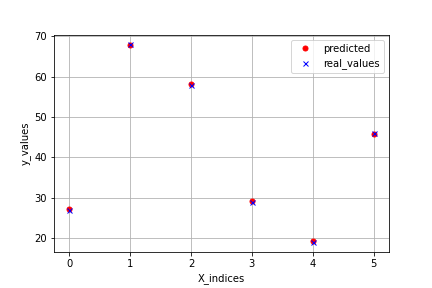
\includegraphics[width=0.8\textwidth]{grad_dec.png}
\end{figure}

At this point, we should note the following points;
\begin{itemize}
\item Learning rate defines the behavior of the gradient decent. If we choose $\eta=0.1$, the iteration simply diverges. Thus choosing an optimal learning rate is an essential task in any deep learning model.

\item Number of epochs is also another factor which effects the approximation. Although it is tempting to consider a large value to get a better approximation, execution time can be a huge hurdle if the model is relatively large.

\item This network is essentially a linear model. We will modify it in a nonlinear fashion using an \textit{activation function} to make it  learn more complex tasks. In fact, introducing an activation function has huge implications on learning task that we will discuss in the next sections. 
 
\end{itemize}



\subsubsection{Gradient Based Learning}
\label{sec:GBL}

In this section, we will generalize the ideas above for any feed forward network  We will closely follow the conventions in \cite{DnnBook}. Lets consider the following notations:
\begin{tcolorbox}
\begin{flushleft}
$w_{jk}^{l} \rightarrow$ weight from the $k^{th}$ neuron in layer $l-1$ to the $j^{th}$ neuron in layer $l$. \\

$b_{j}^{l} \rightarrow$ bias of the $j^{th}$ neuron in layer $l$

$a_{j}^{l} \rightarrow$ activation of the $j^{th}$ neuron in layer $l$
\end{flushleft}
\end{tcolorbox}
A typical fully connected network with L-layer can be seen in the Figure \ref{fig:FCL}. For simplicity, we did not draw all connections.


\begin{figure}[H]
  \centering
  \fbox{\includegraphics[width=0.8\textwidth]{FCL.png}}
  \label{fig:FCL}
\end{figure}
Next we define an activation function. The most commons ones are the followings

\begin{flushleft}
\begin{subequations}

\begin{equation}
\psi(x)=\left\{
        \begin{array}{ll}
            0 & \quad x \leq 0 \\
            x & \quad x > 0
        \end{array}
    \right.
 \quad \rightarrow \text{Rectified linear unit}
\end{equation}

\begin{equation}
\psi(x)=\left\{
        \begin{array}{ll}
            0 & \quad x \leq 0 \\
            1 & \quad x > 0
        \end{array}
    \right.
 \quad \rightarrow \text{Binary step}
\end{equation}

\begin{equation}
\psi(x) =  \sigma(x)=\dfrac{1}{1+e^{-x}} \quad \rightarrow \text{sigmoid}
\end{equation}

\begin{equation}
\psi(x) =  \tanh{x}=\dfrac{1}{1+e^{-2x}} \quad \rightarrow \text{tan hyperbolic}
\end{equation}


\begin{equation}
\psi(x) =  \arctan{x} \quad \rightarrow \text{inverse tangent}
\end{equation}

\end{subequations}
\end{flushleft}
% \begin{figure}[H]
%  \centering
%  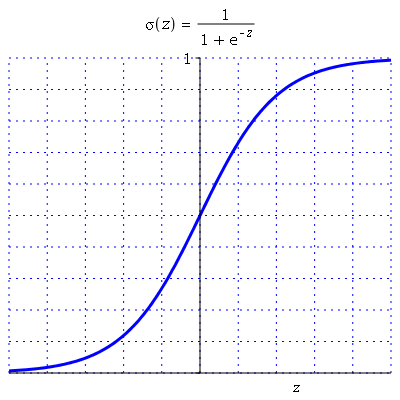
\includegraphics[width=0.5\textwidth]{sigmo.png}
%  \label{fig:sigmo}
%\end{figure}
%
%Note that the $\sigma(z)$ is defined for all real numbers with the range $(0,1)$. 
we define a model by taking a generic activation function $\psi(x)$ as follows: 

\begin{tcolorbox}
\begin{subequations}
\begin{equation}
\label{zwa}
z_{j}^{l} = \sum_{k} w_{jk}^{l}a_{k}^{l-1}+b_{j}^{l}
\end{equation}
\begin{equation}
\label{act}
a_{j}^{l}=\psi(z_{j}^{l})
\end{equation}
where the sum is over the neurons in the $(l-1)^{th}$ layer .
\end{subequations}
\end{tcolorbox}

We will call $z_{j}^{l}$ as an output and $a_{j}^{l}$ as an activation. Relationship between two consecutive layers can be expressed as a matrix multiplication as follows:
\begin{subequations}
\begin{equation}
\begin{bmatrix} 
z_{1}^{l}  \\
z_{2}^{l} \\
..  \\
z_{j}^{l} \\
..
\end{bmatrix} 
=
\begin{bmatrix} 
w_{11}^{l} & w_{12}^{l} & w_{13}^{l} & ... \\
w_{21}^{l} & w_{22}^{l} & w_{23}^{l} & ... \\
.. & .. & .. & .. \\
..& .. &  w_{jk}^{l} & .. \\
..& .. & .. & ..
\end{bmatrix}
\begin{bmatrix} 
a_{1}^{l-1}  \\
a_{2}^{l-1} \\
..  \\
a_{k}^{l-1} \\
..
\end{bmatrix} 
+
\begin{bmatrix} 
b_{1}^{l}  \\
b_{2}^{l} \\
..  \\
b_{j}^{l} \\
..
\end{bmatrix} 
\end{equation}

\begin{equation}
\begin{bmatrix} 
a_{1}^{l}  \\
a_{2}^{l} \\
..  \\
a_{j}^{l} \\
..
\end{bmatrix} 
=
\psi
\begin{bmatrix} 
z_{1}^{l}  \\
z_{2}^{l} \\
..  \\
z_{j}^{l} \\
..
\end{bmatrix} 
\end{equation}
\end{subequations}
In matrix-vector notation, we can write 

\begin{equation}
z^{l} = W^{l}a^{l-1}+b^{l}  
\end{equation}

Note that if there are $\bm{M}$ neurons in $l^{th}$ layer and  $\bm{N}$ neurons in $(l-1)^{th}$ layer, $W$ becomes 
$\bf{MxN}$ matrix. 

Let $m$ and $n$ be the dimensions of the input and output layers. By following a similar path, we will derive the fundamental equations which enable us to approximate a given function $\vec{y}_{n}=f(\vec{x}_{m})$. We should note that this function has a discrete form in practical applications. In other words, we try to optimize the parameters of the architecture to find the best approximate for the data points $(\vec{x},\vec{y})$. Let 
\begin{equation}
C=C(a^{L};y)
\end{equation}
be a generic cost function which we will specify later on. Although $C$ is defined over the last output layer, it is an implicit function of all weights and biases in the architecture. We can re-look at the structure of the last layer in Figure \ref{fig:output}.


\begin{figure}[H]
  \centering
  \fbox{\includegraphics[width=0.5\textwidth]{output.png}}
  \label{fig:output}
\end{figure}


We want to find an expression of the rate of change of the cost function with respect to the weights and biases of the architecture. Lets define a generic error expression: 

\begin{equation}
\delta_{j}^{L} = \dfrac{\partial C}{\partial z_{j}^{L}} 
\end{equation}
Using the chain rule with \ref{act}, we can write
\begin{equation}
\label{fe1}
  \delta_{j}^{L} = \dfrac{\partial C}{\partial a_{j}^{L}} \dfrac{\partial a_{j}^{L}}{\partial z_{j}^{L}} = \dfrac{\partial C}{\partial a_{j}^{L}} \psi'(z_{j}^{L})
\end{equation}  
In vectorial form 
\begin{tcolorbox}
\begin{equation}
\label{FE1}
\delta^{L} = \nabla_{a} C \odot  \psi'(z^{L})
\end{equation}
\end{tcolorbox}
where $\odot$ represents component-wise (Hadamard) product with the gradient \\
$\nabla_{a}C =
\begin{bmatrix} 
\dfrac{\partial C}{\partial a_{1}^{L}} &, \dfrac{\partial C}{\partial a_{2}^{L}} &,.. &, \dfrac{\partial C}{\partial a_{n}^{L}} \\
\end{bmatrix}
^{T} 
$
Once $z^{L}$ is computed through forward pass, (\ref{FE1}) can be evaluated with a prescribed cost function. In other words, this information is sufficient to update the weights and biases in the last layer. Now, we will propagate this error all the way back to the second layer. Lets look at the rate of change of the cost function with respect to the output $z_{j}^{l}$. Carefully note that all neurons $z^{l+1}$ in the $(l+1)^{th}$ layer is dependent on $z_{j}^{l}$. Thus the following relations holds:
$$
\delta_{j}^{l} = \dfrac{\partial C}{\partial z_{j}^{l}} =  \mathlarger{\sum}_{k} \dfrac{\partial z_{k}^{l+1}}{\partial z_{j}^{l}} \dfrac{\partial C}{\partial z_{k}^{l+1}} = \mathlarger{\sum}_{k} \dfrac{\partial z_{k}^{l+1}}{\partial z_{j}^{l}}\delta_{k}^{l+1}
$$  
If we rewrite the relation (\ref{zwa}), $z_{k}^{l+1} = \displaystyle{\sum_{j} w_{kj}^{l+1}a_{j}^{l}+b_{k}^{l+1} = \sum_{j} w_{kj}^{l+1}\psi(z_{j}^{l})+b_{k}^{l+1}} $, we obtain $\dfrac{\partial z_{k}^{l+1}}{\partial z_{j}^{l}} = 
w_{kj}^{l+1}\psi'(z_{j}^{l})$. This implies 

\begin{equation}
\delta_{j}^{l} = \mathlarger{\sum}_{k} w_{kj}^{l+1}\delta_{k}^{l+1}\psi'(z_{j}^{l})
\end{equation}
In vectorial form, we have 
\begin{tcolorbox}
\begin{equation}
\label{FE2}
\delta^{l} =  (W^{l+1})^{T}\delta^{l+1} \odot \psi'(z^{l})
\end{equation}
\end{tcolorbox}
Our main goal is to propagate the error on the previous layers to update the weights and biases. From (\ref{zwa}), we can write


\begin{tcolorbox}
\begin{equation}
\label{FE3}
\dfrac{\partial C}{\partial b_{j}^{l}} = \dfrac{\partial z_{j}^{l}}{\partial b_{j}^{l}}  \dfrac{\partial C}{\partial z_{j}^{l}} = 1\cdot \delta_{j}^{l}
\end{equation}

\begin{equation}
\label{FE4}
\dfrac{\partial C}{\partial w_{jk}^{l}} = \dfrac{\partial z_{j}^{l}}{\partial w_{jk}^{l}}  \dfrac{\partial C}{\partial z_{j}^{l}} = a_{k}^{l-1} \delta_{j}^{l}
\end{equation}
\end{tcolorbox}

Using these last two equations in the light of (\ref{FE1}) and (\ref{FE2}), we can describe one cycle forward pass and back prorogation as follows:

\begin{algorithm}{}\label{alg:GD}
      \caption{Gradient Decent for a Feed Forward Network}
      \begin{algorithmic}
      \State Set input data $\vec{x}_{m}$ and learning rate $\eta$ 
      \State Assign initial values to all weights and biases. 
      \State \textbf{Feed Forward}
       \For {$l=2,3...L$}
       \State $a^{l} =\psi( W^{l}a^{l-1}+b^{l}) $
       \EndFor
       \State Compute the output loss and update the last layer parameters
       \State $\delta^{L} = \nabla_{a} C \odot  \psi'(z^{L})$       
       \State $W^{L} \leftarrow W^{L} -\eta \delta^{L}(a^{L-1})^{T} $
       \State $b^{L} \leftarrow b^{L} -\eta \delta^{L} $
       \State \textbf{Back Propagation}
       \For {l = L-1, L-2, ...2}
       \State $\delta^{l} =  (W^{l+1})^{T}\delta^{l+1} \odot \psi'(z^{l})$
       \State $W^{l} \leftarrow W^{l} -\eta \delta^{l}(a^{l-1})^{T} $
       \State $b^{l} \leftarrow b^{l} -\eta \delta^{l} $
       \EndFor
      \end{algorithmic}
    \end{algorithm} 
In the back propagation step, $\delta^{l}(a^{l-1})^{T}$ is the matrix form of the component-wise expression  (\ref{FE4}). Above algorithm is the description for a single epoch and a single data point. 

Note that we use a generic learning rate $\eta$ for all layers but in practice one can use a parameter-based learning rate and adjust the learning rate layer-wise or parameter-wise. For example, one of the most popular optimization methods in deep learning ADAM(Adaptive Moment Estimation)\cite{adam} computes adaptive learning rates for each parameter but trade off in this scheme is that it requires more time to train comparing to other methods.

\newpage
\begin{flushleft}
\textbf{ Some comments on the activation function}
\begin{enumerate}
\item Let's consider the equation (\ref{FE1}) with the sigmoid function. As we can see fro the figure (\ref{fig:sigmo}), the range of $\sigma$ is $[0,1]$. Thus if $\sigma(z_{j}^{L})\approx 0$ or $1$, its derivative at this point is near flat, i.e, $\sigma'(z_{j}^{L})\approx 0 $. Thus the weight associated with this node most likely changes very slowly in gradient decent or we say learns slowly. This type of neurons are called saturated or near saturation. 
%Similar discussions hold also for the equation (\ref{FE2}) which pertains to the early layers. This problem is also known as learning slowdown. 
 \begin{figure}[H]
  \centering
  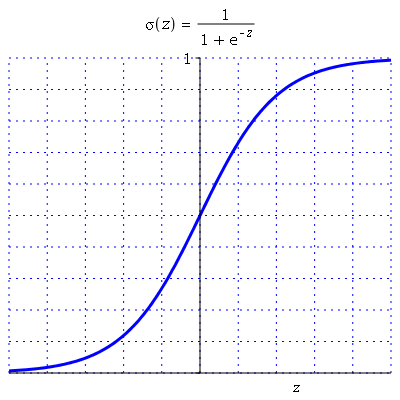
\includegraphics[width=0.5\textwidth]{sigmo.png}
  \label{fig:sigmo}
\end{figure}

\item In the light of the same discussion, let's take the equation (\ref{FE2}) which we we utilize to update the weights and biases at the corresponding layers. Notice that the saturation effect in the last layers may propagate back to the early layers and cause neurons to learn very slowly or even completely stop the parameter updates. The effect can be observed more clearly especially in the first layers of very deep architectures. This problem is known as the \textit{vanishing gradient problem}. That being said, we should note that the others terms in (\ref{FE1}) can balance the saturation problem and the model may not suffer from vanishing gradient. Thus this phenomena requires careful mathematical analysis.

\item One way to avoid saturation problem would be to define an activation function whose derivative does not vanish. Probably the most common activation function used in this sense is the rectified linear unit (Relu) $\psi(x)=max(x,0)$ which is always positive with a positive derivative. In practice, Relu is almost the best choice. See figure (\ref{fig:relu}).

 \begin{figure}[H]
  \centering
  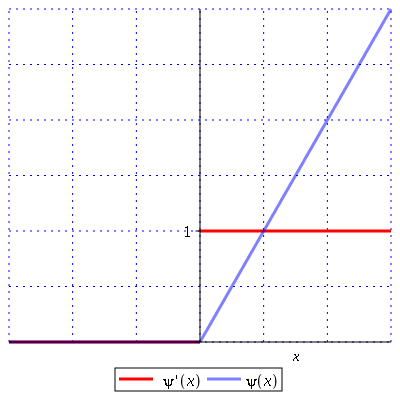
\includegraphics[width=0.5\textwidth]{relu.png}
  \label{fig:relu}
\end{figure}

\end{enumerate}
\end{flushleft}


We have not discussed a specific form of the cost function to this point. Assume that we have data set containing $N_{p}$ data points of the forms 
\begin{equation}
\mathcal{D} = \{(\vec{x^{i}},\vec{y^{i}} )\}_{i=1}^{N_{p}}
\end{equation}
These are predefined input and output values. We prefer to use vector notation because we usually deal with multidimensional input and output. We will use this data set to update the learnable parameters of the architecture. In other words, we train the model using this data set. Thus we will call $\mathcal{D}$ as a \textit{training set}. A proper cost function for this data set must be of the following form 
\begin{equation}
\label{cf}
C = \sum_{i=1}^{N_{p}}C^{(i)}(\vec{y^{i}};a^{(i)L})
\end{equation}
where $a^{(i)L}$ is the output activation or predicted value for $\vec{x^{i}}$ and the form of $C^{(i)}$ is to be specified. One common cost function is the mean-square error  function defined as

\begin{equation}
\label{CF}
C = \dfrac{1}{2N_{p}}\sum_{i=1}^{N_{p}} \|  \vec{y^{i}}-a^{(i)L}   \|^{2}
\end{equation}
where the vector norm $\|  \|$ can be defined as the Euclidean distance, i.e, 

$$\|  \vec{y^{i}}-a^{(i)L}   \|^{2} = \sum_{k=1}^{n} (y^{i}_{k}-a^{(i)L}_{k})^{2}   $$

In gradient decent algorithm, we must compute the gradient of the cost function $\nabla_{a} C $ to evaluate the term $\delta^{L} = \nabla_{a} C \odot  \psi'(z^{L})$. Using (\ref{cf}), we have 

\begin{equation}
\nabla_{a} C =  \sum_{i=1}^{N_{p}}\nabla_{a}C^{(i)}
\end{equation}
Once we have this value, we can then enter the loop and update the parameters. However if $N_{p}$ is very large, i.e. training set consists of large number of samples, finding the exact value of the gradient is not feasible from computational cost viewpoint. So the most common approach is to update the parameters after some specified value $M$ such that $M < N_{p} $. This approach is called \textit{stochastic gradient decent }.In mathematical terms,   
   
\begin{equation}
\label{eq:bgd}
\nabla_{a} C =  \sum_{i=1}^{N_{p}}\nabla_{a}C^{(i)} \approx \sum_{i=1}^{M}\nabla_{a}C^{(i)}
\end{equation}
$M$ is called the \textit{batch} size and along with the learning rate this is another parameter which should be taken into account in training stage. 



\begin{flushleft}
\textbf{Cross Entropy Cost Function} \\
Let's consider the first example in (\ref{mt}) with an activation $\psi(x)$. If we rewrite (\ref{fe1}) for a generic data point $(\vec{x},\vec{y})$
\begin{equation}
\delta_{j}^{L} = \dfrac{\partial C}{\partial a_{j}^{L}} \dfrac{\partial a_{j}^{L}}{\partial z_{j}^{L}} = \dfrac{\partial C}{\partial a_{j}^{L}} \psi'(z_{j}^{L}) = (a_{j}^{L}-y_{j})\psi'(z_{j}^{L})
\end{equation}

If we employ this result in (\ref{FE4}) for the last layer we obtain

\begin{equation}
\label{VG}
\dfrac{\partial C}{\partial w_{jk}^{L}} =  a_{k}^{L-1} \delta_{j}^{L} = a_{k}^{L-1}(a_{j}^{L}-y_{j})\psi'(z_{j}^{L})
\end{equation}

In the discussion above, we see that the term $\psi'(z_{j}^{L})$ can lead to vanishing gradient problem. One idea would be to use the rectified linear unit as an activation function. Another approach is to define a cost function which can eliminate the derivative term in (\ref{VG}). Let's define so called \textit{cross entropy} cost function
along with sigmoid activation. Again for a generic point $(\vec{x},\vec{y})$
\begin{equation}
\label{CE}
C = -\sum_{j} \Big[ y_{j}\ln(a_{j}^{L})+(1-y_{j})\ln(1-a_{j}^{L}) \Big] 
\end{equation} 

where $a_{j}^{L} = \sigma(z_{j}^{L})$. First note that sigmoid function satisfies $\sigma'(x)=\sigma(x)(1-\sigma(x))$. From here, $$ \dfrac{\partial C}{\partial a_{j}^{L}} = -\dfrac{y_{j}}{a_{j}^{L}} + \dfrac{1-y_{j}}{1-a_{j}^{L}} = -\dfrac{y_{j}}{\sigma(z_{j}^{L})} + \dfrac{1-y_{j}}{1-\sigma(z_{j}^{L})} = \dfrac{\sigma(z_{j}^{L})-y_{j}}{ \sigma(z_{j}^{L})(1-\sigma(z_{j}^{L}))} = \dfrac{\sigma(z_{j}^{L})-y_{j}}{ \sigma'(z_{j}^{L}) }$$

If we plug this result into (\ref{VG}), we obtain 

\begin{equation}
\label{eq:ce}
\dfrac{\partial C}{\partial w_{jk}^{L}} =  a_{k}^{L-1} \delta_{j}^{L} = a_{k}^{L-1}(a_{j}^{L}-y_{j})
\end{equation}
Notice that this last expression is free from the derivative term. Thus it theoretically avoids learning slow down.
\end{flushleft}
\begin{flushleft}
\textbf{Softmax Layer} \\
Assume that instead of using an activation function ,we define another type of output layers of the form
\begin{equation}
a_{j}^{L} = \gamma(z_{j}^{L}) =  \dfrac{e^{z_{j}^{L}}}{\sum_{k}e^{z_{k}^{L}}}
\end{equation}
$\gamma$ is called a \textit{softmax} function. We can see that $\gamma$ is monotonically increasing, positive and less than 1. Moreover $\sum_{j}\gamma(z_{j}^{L})=1$.Thus, we can consider the range of $\gamma$ as a probability distribution. In other words, the output of softmax layer can be interpreted as a probability vector. For example, image classification problems, it is common to label different categories with number tags such as 'A':1, 'B':2, 'C':3  and set the correct output as $A:[1,0,0]$, $B:[0,1,0]$, etc. So if the model endowed with softmax outputs a vector such as $[0.90,0.08,0.02]$, we interpret that the input is most likely A and less likely C. Without softmax, the entries of this vector are real numbers and the maximum entry is taken as the predicted value. Notice that softmax provides a nice way to interpret the predictions from probability point of view. 

It is very common to employ logarithmic softmax with negative log-likelihood cost function 

\begin{equation}
C = -\ln(\gamma(z_{j}^{L}))
\end{equation} 

and partial derivatives related to weight and biases gives a similar result to (\ref{eq:ce}). One can also use softmax along with the cross entropy cost.
\end{flushleft}







\section{Convolution Neural Networks(CNN)}
\label{CNN}

In this section, we will introduce the basic principles of another neural network model, convolutional neural networks(CNN). CNN model are commonly applied for image analysis problems. In the previous section, we discussed DNN models where each neuron are essentially connected to each other in the architecture. This actually means we dont assume any meaningful connection between the neurons. A CNN models aims to explore possible hidden connections in the input data and by this way enables the architecture to learn with a more \textit{regularized} way. 

\subsection*{Introduction}
\label{introCNN}
Let's start with the formal definition of the convolution operation. Convolution is a special integral transform. Let $f$ and $b$ be two functions. " f convolution g " is a function defined as

\begin{equation}
\label{eq;conv}
(f*g)(x) = \int_{-\infty}^{\infty} f(\tau)g(x-\tau)d\tau
\end{equation}
Geometrically, we first reflect the function $g(\tau)$ to $g(-\tau)$ and add a time offset so that we obtain $g(t-\tau)$ .We then multiply $g(t-\tau)$ with $f(\tau)$, vary $t$ from $-\infty$ to $\infty$ and compute the integral over all $t$'s where both function are non-zero. In practical application, we can use define a discrete a convolution in 2D as follows:

\begin{equation}
\label{eq;dconv}
(f*g)(x,y) = \sum_{i,j} w_{ij}f(\tau_{i},\tau_{j})g(x-\tau_{i},y-\tau_{j})
\end{equation}
where $w_{ij}$ are the integral weights.

Let's consider a concrete example to illustrate how (\ref{eq;dconv}) can be used in image processing. Let the function $f$ represents an $mxn$ pixel image. So $f(x_{i},y_{j})$  is the pixel value at $(i,j)$ location. We will $g(x,y)$ as a \textit{kernal} function. Assume that as a discrete function $g(x,y)$ has $3x3$ pixel support size. In this case, for a specific pixel location,  the sum in (\ref{eq;dconv}) is performed over this $3x3$ region. Similar to the continuous case, we start with the upper left most pixel, apply 3x3 discrete convolution and slide $g$ to the next pixel and perform the same operation. When we scan the entire pixels, the result is essentially another image. Here, the sliding amount is called the \textit{stride} size while the $3x3$ is called the \textit{filter size}. An illustrative figure can be seen below.

 \begin{figure}[H]
 \label{pic:conv}
  \centering
  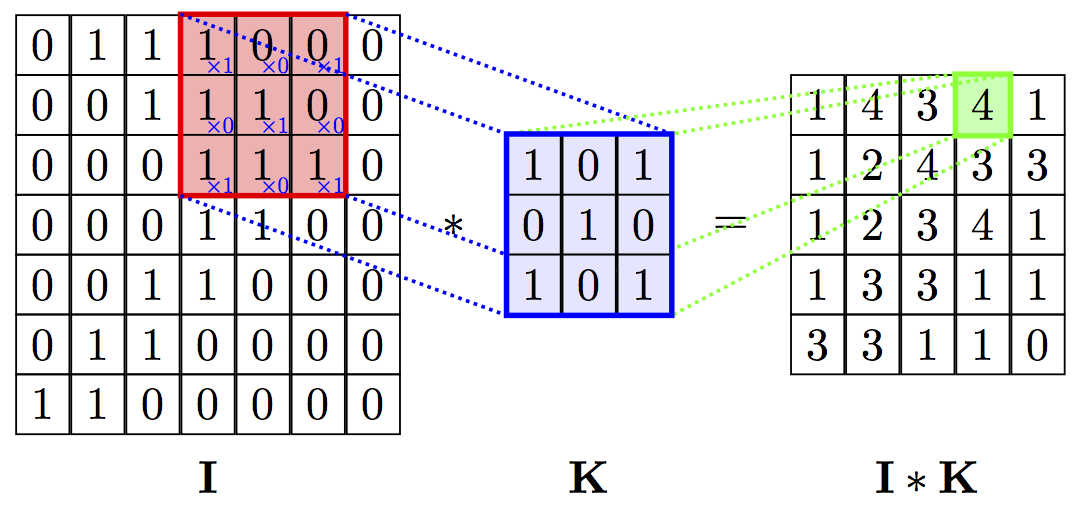
\includegraphics[width=0.5\textwidth]{conv.png}
\end{figure}

The convolution or filtering operation plays a central role in image processing. Discrete kernels are used for noise removal, edge detection, image enhancement and so many other image processing operations \cite{IP}. For example, following kernels can be used as edge detectors. 

 \begin{figure}[H]
 \label{fig:edge}
  \centering
  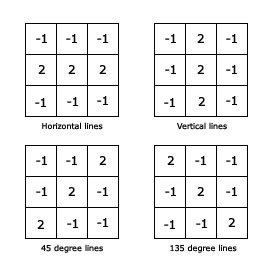
\includegraphics[width=0.5\textwidth]{detec.png}
\end{figure}

There are some details in the implementation of image filters such as zero padding, wrapping, reflection etc but we will not go through the details. We should however mention the following formula concerning the output dimension after the convolution. For a square kernel of size $kxk$, and image of size WxW with padding $p$, stride $s$, the output image is of the size 
$$
W_{out} = \dfrac{W-k+2p}{S}+1
$$ 

The kernels in (\ref{fig:edge}) are specifically designed for edge detection. However we can claim that any type of filter applied to an image reveals \textit{some pattern} even if it is qualified as a meaningful pattern. 

CNN models use the kernels to explore the features in a picture in a more systematic way but the major difference is that the kernels are determined by the learnable parameters what we call \textit{shared weights} which don't have prescribed values but evolve over the course the training. Let's  go through the details.   


CNNs have three major components; local receptive fields, shared weights and a pooling layer. Shared weights are different type of kernels and the local receptive field is the portion of the image where we apply the kernel. Carefully note that even though we tend to think the image as $mxn$ pixel size, we in fact have $m\cdot n$ input neurons to be passed to the architecture. In CNN models, convolution operation is usually followed by an \textit{pooling} operation where we further condense the convoluted information. A visial structure of CNN can be seen in figure (\ref{fig:cnn}). (Source https://vinodsblog.com).

 \begin{figure}[H]
 \label{fig:cnn}
  \centering
  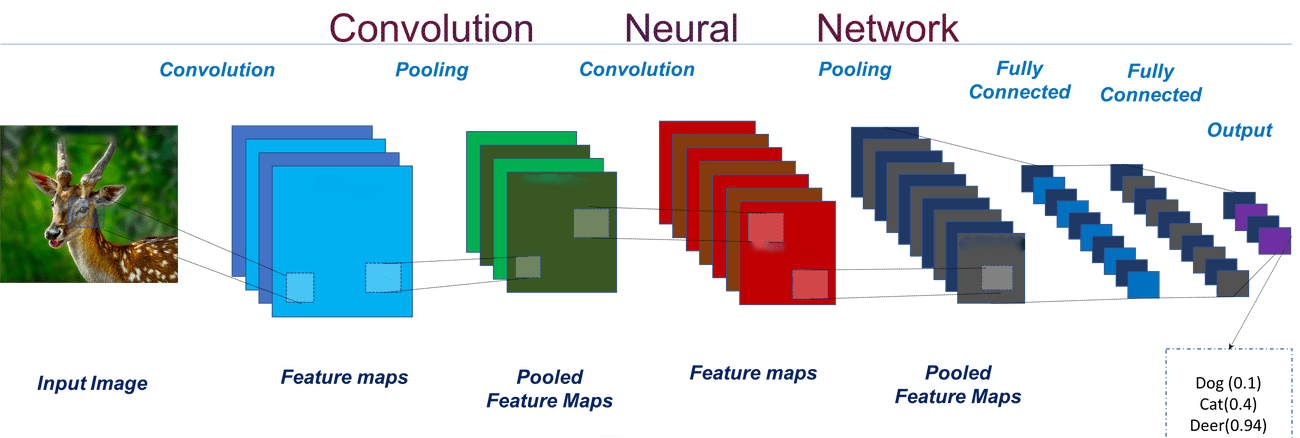
\includegraphics[width=1.1\textwidth]{CNN-2.png}
\end{figure}

Let's formally define how to apply convolution operation in a CNN model. In convolution layers, we have convolution operation instead of matrix multiplication, which we can define as follows

\begin{equation}
\label{eq:dcon}
z_{x,y}^{l+1} = w^{l+1}*\psi(z_{x,y}^{l}) + b_{x,y}^{l+1} = \sum\limits_{a=1}^{k} \sum\limits_{b=1}^{k} w_{a,b}^{l+1}\psi(z_{x-a,y-b}^{l})+b_{x,y}^{l+1}
\end{equation}
where $w$ is the $kxk$ kernel at the $l^{th}$ layer, i.e, $kxk$ matrix with entries $w_{a,b}^{l}$. The output image of the convolution operation is called a \textit{feature map}. Note that the kernel $w$ is a parameter which is same for the corresponding feature map but different for the others. As for the bias, we can use one bias per convolution filter (\textit{tied bias}) or one bias for eaach kernel location(\textit{untied bias}). We used untied bias here. Now assume that we have a gray scale image of size of size $50x50$. If we prescribe 7 feature maps with $3x3$ kernels then we have $ 7x(3x3 + 1) = 70 $ parameters with tied bias. Note that for a color image with 3 color channels, we have   $7(3x3x3+1) = 196 $ parameters. The output size of each feature map with zero padding stride 1 becomes $\dfrac{50-3+0}{1}+1 = 48 $. Convolution is followed by a pooling operation which reduce the size of convolution output with an operation called pooling. The most common ones are max pooling and L2 pooling which we define as 

\begin{subequations}
\begin{equation}
z_{i,j} = max\{z_{i+n-1,j+n-1} : 1\leq n \leq p \}  \quad\quad \text{max pooling}
\end{equation} 

\begin{equation}
z_{i,j} = \sqrt{\sum\limits_{n=1}^{p} \sum\limits_{n=1}^{p} z_{i+n-1,j+n-1}^{2}} \quad\quad \text{L2 pooling}
\end{equation}
\end{subequations}
where $p$ is the pooling size. Max pooling outputs  the maximum element in $pxp$ pooling region while L2 pooling computes the L2 average. Output dimension of a pooling operation can be found as follows:
$$
W_{out} = \dfrac{W-p}{S}+1
$$
where $W$ is the input size, $p$ is the kernel size and $S$ is the stride.
Complete picture can be seen in figure (\ref{fig:convp}).

\begin{figure}[H]
 \label{fig:convp}
  \centering
  \includegraphics[width=1.1\textwidth]{convpool.png}
\end{figure}

\subsection{Back Propagation in CNN Models}

In this section, we will derive the fundamental equations of backpropagation in CNN models. Let's define 

\begin{equation}
\label{eq:cnnE1}
\delta_{x,y}^{l} = \dfrac{\partial C}{\partial z_{x,y}^{l}} 
\end{equation} 
for a generic cost function. Using the chain rule and (\ref{eq:dcon}), we can write 

\begin{equation}
\delta_{x,y}^{l} = \dfrac{\partial C}{\partial z_{x',y'}^{l+1}} \dfrac{\partial z_{x',y'}^{l+1}}{\partial z_{x,y}^{l}}
=
\sum\limits_{x'} \sum\limits_{y'} \delta_{x',y'}^{l+1} \dfrac{\partial }{\partial z_{x,y}^{l}} 
\Big( \sum\limits_{a} \sum\limits_{b} w_{a,b}^{l+1}\psi(z_{x'-a,y'-b}^{l})+b_{x',y'}^{l+1} \Big)
\end{equation} 
Note that the derivative term above is 0 expect the indexes satisfying $x'-a=x$ and $y'-b=y$, i.e.,  $a = x'-x, b = y'-y $. Using the definition of the convolution (\ref{eq:dcon}), we have

\begin{equation}
\label{eq:cnnE2}
\delta_{x,y}^{l} =  \sum\limits_{x'} \sum\limits_{y'} \delta_{x',y'}^{l+1} w_{x'-x,y'-y}^{l+1}\psi'(z_{x,y}^{l}) = 
\delta^{l+1}*w_{-x,-y}^{l+1} \psi'(z_{x,y}^{l})
\end{equation}
Sometimes, it is written $w_{-x,-y}= ROT180(w_{x,y})$ Here ROT180 represent the 180 degree rotation of the kernel. If start indexing $w$ from the middle element entry, $w_{-x,-y}$ can be found by rotating the same kernel 180 degree about $(0,0)$ index. We then compute the partial derivatives using (\ref{eq:cnnE2}).
$$
 \dfrac{\partial C}{\partial w_{a,b}^{l}} =  \sum\limits_{x} \sum\limits_{y} \dfrac{\partial C}{\partial z_{x,y}^{l}} \dfrac{\partial z_{x,y}^{l}}{\partial w_{a,b}^{l}} 
=
\sum\limits_{x} \sum\limits_{y} \delta_{x,y}^{l} \dfrac{\partial }{\partial w_{a,b}^{l}} 
\Big( \sum\limits_{a'} \sum\limits_{b'} w_{a',b'}^{l}\psi(z_{x-a',y-b'}^{l-1})+b_{x,y}^{l} \Big)
= 
$$
$$\sum\limits_{x} \sum\limits_{y} \delta_{x,y}^{l} \psi(z_{x-a,y-b}^{l-1}) = \delta_{a,b}^{l}*\psi(z_{-a,-b}^{l-1})$$
So we have 
\begin{equation}
\label{eq:cnnE3}
 \dfrac{\partial C}{\partial w_{a,b}^{l}}  = \delta_{a,b}^{l}*\psi(z_{-a,-b}^{l-1})
\end{equation}
and similarly 
\begin{equation}
\label{eq:cnnE4}
 \dfrac{\partial C}{\partial b_{a,b}^{l}}  = \delta_{a,b}^{l}
\end{equation}
We can close this section with an interesting note. As we see from the construction, we do not pre-assign any specific kernel type (Prewitt, Sobel, Gabor filters etc) to reveal some patters in the input images. However it is observed that as we train the architecture, shared weights are learning to reveal meaningful \textit{patterns }. In particular early layers learns basic shapes such as vertical, horizontal lines while the next layers learn more compact patters such as cars, ships, mountains etc.

\section{Overfitting and Underfitting}
\label{sec:overunder}

Typical deep neural network with dense and convolutional layers contain massive number of learnable parameters. For example, let's consider one of the first large scale CNN model Alexnet \cite{alexnet} which can be seen in figure \ref{fig:alex}. It has eight layers; five convolutional layers, some of them followed by max-pooling layers, and three fully connected layers. Total number of weights in Alexnet is $\mathbf{60,954,656!}$. It was the winner of the Large Scale Visual Recognition Challenge in 2012 \cite{imagenet} where the task is to classify 150,000 images in 1000 different categories. The training dataset is composed of 1.2 million images. 

\begin{figure}[H]
 \label{fig:alex}
  \centering
  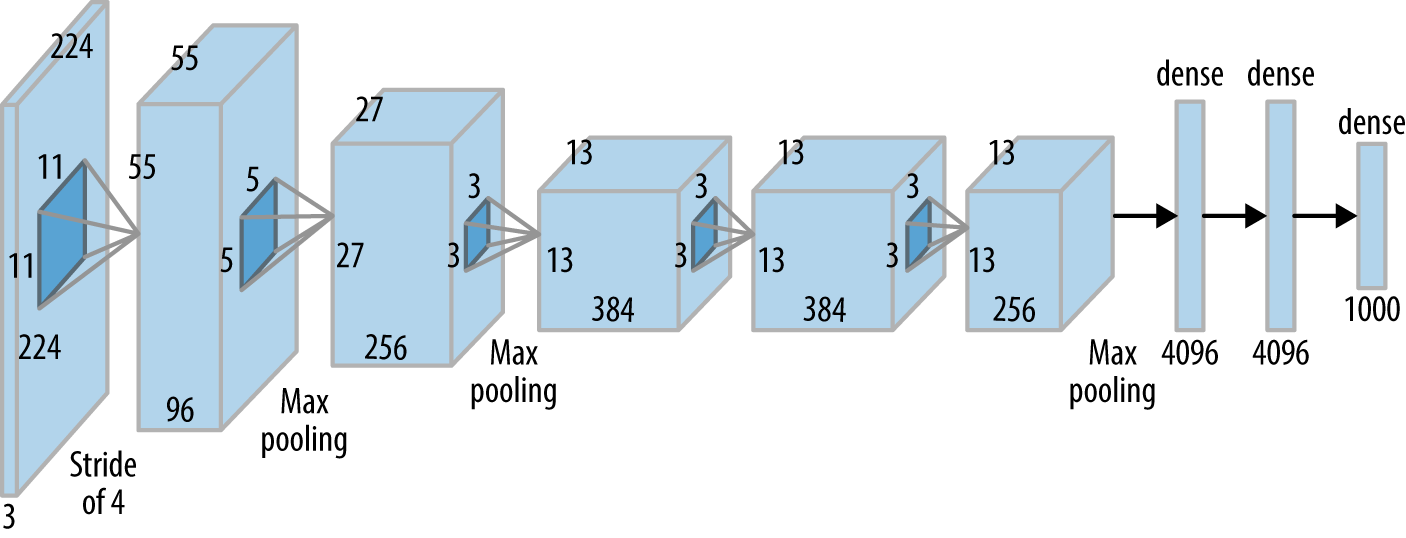
\includegraphics[width=1.1\textwidth]{alex.png}
\end{figure}
So in mathematical terms, we are using millions of free parameters to solve an approximation problem. Due to the massive number of parameters, the model can quickly learn or memorize all sorts of details of the training data set but may not be able to generalize to or perform well on a different data which was not introduced to the model. This problem is known as \textit{overfitting}. In any deep neural architecture, this problem must be taken with a great care. In the same sense, we can also define \textit{underfitting} which is the case where the model can not capture the underlying structure of the data. There are various ways to detect whether a model is overfitting. One of the most effective way is to monitor the accuracy on training and testing set. \textit{If the validation accuracy is considerably lower than the training accuracy}, this means that the model is failing to generalize beyond the training data set. See the figure below.

\begin{figure}[H]
 \label{fig:overfit}
  \centering
  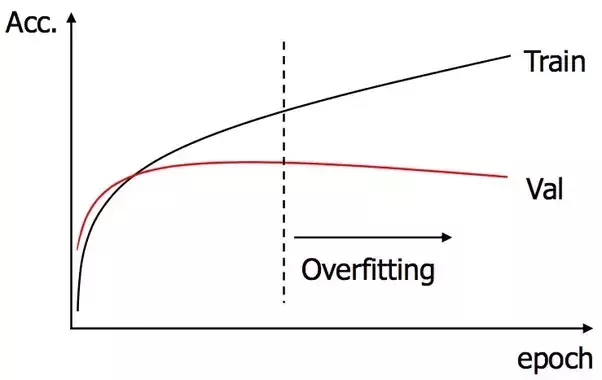
\includegraphics[width=0.4\textwidth]{overfit.png}
\end{figure}

In fact one obvious way to tackle with overfitting problem, which we implicitly discussed throughout this report, is to split the data set into training and validation subsets. There is no agreed-opon ratio but 80\% vs 20\% splitting scheme is very common. We then train the data on training data set and monitor the accuracy on the validation set. In addition, we can consider a third subset where we can tune the other parameters such as the number of epochs, learning rate. We will discuss several methods how to avoid overfitting problem along with how to improve the ability of learning of a model.

\section{Improving Neural Networks}
In the previous sections, we already discussed several methods which can enhance the architecture's capacity to learn on a given data set. In this section, we further introduce various ways to improve the quality of a model. We should note that our ultimate goal is to \text{efficiently} build a model  which can make accurate predictions in \text{the most general setting}. We can collectively call these techniques as \text{regularization}. These techniques enable us to train faster, eliminate overfitting and better generalize to the new situations. Note that regularization is an huge active research area . Thus this section should be taken as a brief and incomplete overview of the existing techniques. For an extensive overview, refer to \cite{prac}.



\subsection{Momentum Based Gradient Decent}
In the previous section, we have seen that the ultimate goal of the gradient decent is to gradually converge to a point which minimizes the cost function and we tried to achieve this taking small steps in the direction of the negative gradient. From theoretical perspective, this is a very challenging problem. Because the cost function essentially operates in a very high dimensional space. We mentioned that  the Alexnet has around 60M parameters so the cost function represents a $60M$-dimensional surface. The primary challenge here is to distinguish between the local minimum and the global minimum since we are dealing with a \textit{nonconvex} surface.  Stochastic gradient decent (SGD) may help us to tackle with this problem for relatively \text{shallow local minimum} points but one should introduce different methods to achieve further results for \textit{deep local minimum} points \cite{fund}.

Momemtum-based gradient decent which is motivated by Hessian approximation to the cost function  addresses this problem. We will not further pursue this topic here but just describe the procedure. Idea is to modify the gradient decent with a \textit{momemtum variable}. For a generic quantity of interest $w$,


\begin{equation}
\begin{split}
v^{(n)} = \mu v^{(n-1)} + \eta \nabla C \\
w^{(n)} = w^{(n-1)} + v^{(n)}
\end{split}
\end{equation}
where $\mu$ is momentum variable and $\eta$ is the learning rate. Roughly speaking momentum parameter smooths the step size taken in the direction of the gradient. It also dramatically decreases the training time by quickly minimizing the cost function. Modern optimization schemes such as ADAGrad, RMSProp, ADAM either directly use momentum parameter or take advantage of similar approaches. 

\subsection{Regularization}

In regularization technique, we add a penalty term to the usual cost function $C_{0}$ as follows

\begin{subequations}
\begin{equation}
\label{eq:l2}
C = C_{0} + \dfrac{\lambda}{2n}\sum\limits_{w}\|w\|^{2}_{2}
\end{equation}

\begin{equation}
\label{eq:l1}
C = C_{0} + \dfrac{\lambda}{2}\sum\limits_{w}\|w\|_{1}
\end{equation}
\end{subequations}
(\ref{eq:l2}) called \textit{L2}(or Ridge regression) regularization and (\ref{eq:l1}) is called \textit{L1} regularization. Here $\lambda$ is the regularization parameter and $n$ as the number of training data points. If the gradient decent is applied to (\ref{eq:l2}) for a generic parameter $w$, we can see 

\begin{equation}
\label{eq:sgdL2}
w^{(k+1)} = (1-\dfrac{\eta \lambda}{n})w^{(k)} - \eta \dfrac{\partial \nabla C}{\partial w} 
\end{equation}
The term $1-\dfrac{\eta \lambda}{n}$ is called the \textit{weight decay}. From (\ref{eq:sgdL2}), it is clear that the weight decay makes the weight smaller.  We have seen that the forward pass is govern by the equation
$$
z^{l} = \psi(W^{l}a^{l-1}+b^{l})
$$
By decreasing the weights, we essentially reduce the effect of the activation function,i.e, we don't allow the model to fully utilize its free variables. So we interpolate the data with less complex function. This, in turn, effectively reduces overfitting. 

\subsection{Dropout}
One of the most effective regularization technique is to randomly drop some of the nodes during the training, for example in each epoch. The idea is to prevent the model to learn over certain nodes and spread the learning procedure across the architecture.  This technique is called \textit{dropout}. However we do not change the main skeleton of the model by dropping the neurons but zero out the parameters of the corresponding neurons. 
Dropout is generally implemented in a random fashion. At each epoch, individual neurons are either dropped out of the model with probability 1-p or or kept with probability p so that we obtain a simplified model; incoming and outgoing edges to a dropped-out neurons are also removed. Figure \ref{fig:drop}

\begin{figure}[H]
 \label{fig:drop}
  \centering
  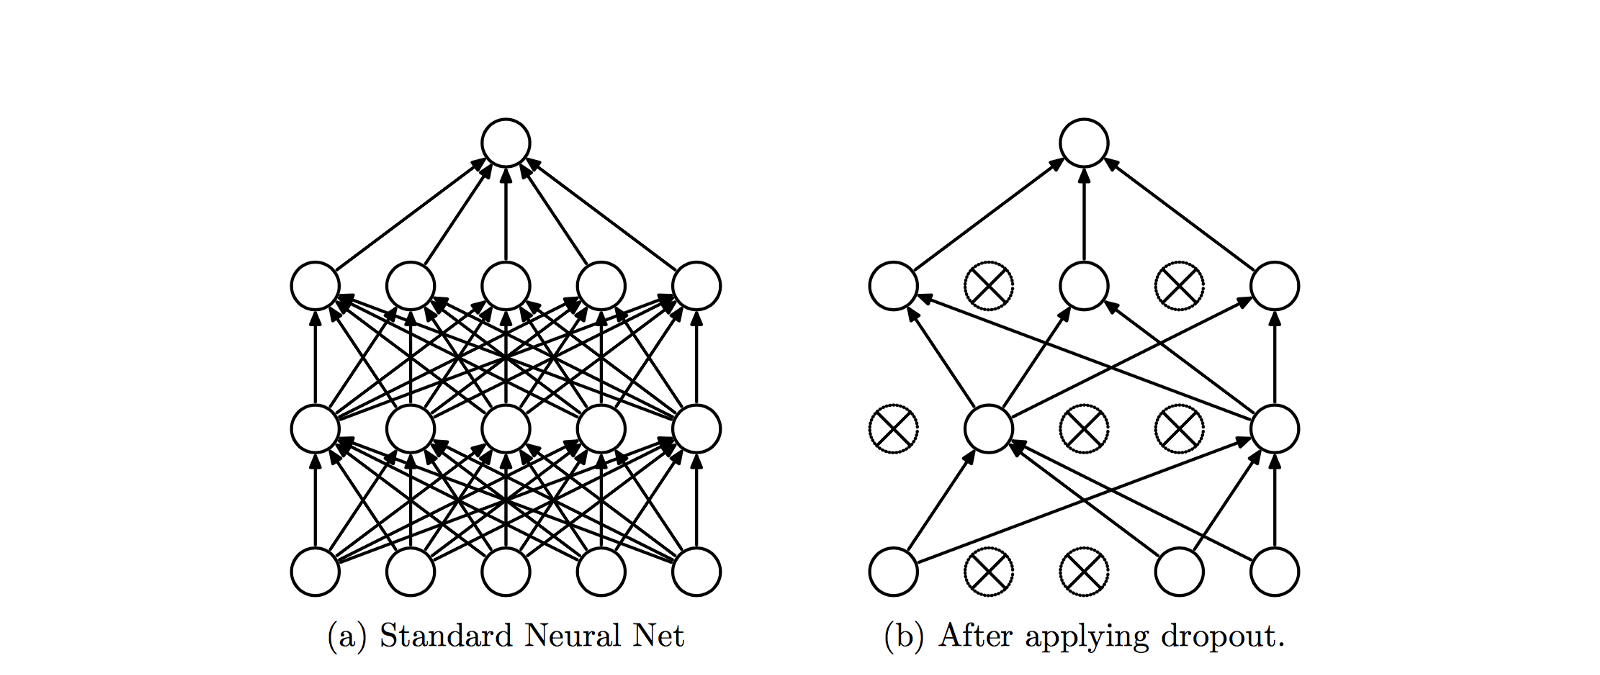
\includegraphics[width=1\textwidth]{dropout.png}
\end{figure}
\textit{Carefully note that all neurons are present when we start testing the accuracy of the model in the validation stage. Thus dropout is the property of training not validation. Because of that, Pytorch provides two modes of the model, training mode where we apply dropout, batch normalization and evaluation mode where we calculate the plain predictions.}



\subsection{Early Stopping}
Let's reexamine the figure (\ref{fig:overfit}) again. 
\begin{figure}[H]
 \label{fig:overfit2}
  \centering
  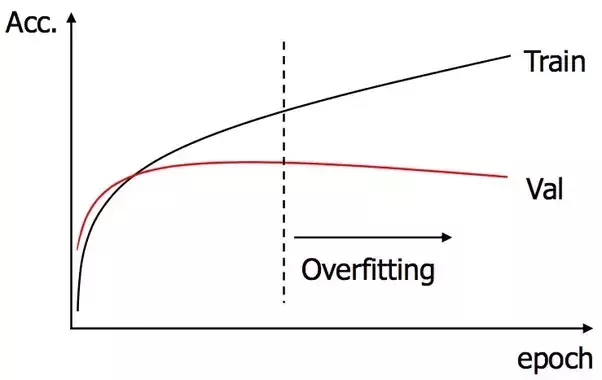
\includegraphics[width=0.4\textwidth]{overfit.png}
\end{figure}
It is obvious that the model is overfitting beyond the dashed line. Having an observation like this gives us a very cheap way to set an optimal number of epochs. Or we can set a threshold on the acceptable difference between the training and validation accuracy or loss and stop whenever the model reaches that threshold. This is called \textit{early stopping}. In fact, the graph above is one of the essential dynamics of a network that we should monitor in training stage.

%\subsection{Weight Initialization}
\subsection{Preprocessing}
Since any kind of data contains noise and random variations, it is very common to perform preprocessing on the data set before the training. For example, resizing to a fixed size and normalizing the data using a fixed mean and standard deviation is an essential practice in computer vision tasks. One common practice is to use ImageNet statistics for normalization;
\begin{align*}
mean = [ 0.485, 0.456, 0.406 ] \\
std = [ 0.229, 0.224, 0.225 ]
\end{align*} 
for each color channel accordingly and the pixel values are scaled to $[0,1]$. It has been shown that the normalizing the input data helps the model to learn faster and efficiently \cite{lecun}. 


\subsection{Shuffling}

We discussed the stochastic gradient decent in section (\ref{sec:GBL}) and introduced the notion of batch in (\ref{eq:bgd}). So we pass a batch of images to the architecture, compute the loss and update the parameters and repeat the process until we process all the training data. We called this one epoch loop. One of the very effective technique to avoid overfitting and better train the model is to shuffle the data in \textit{each epoch} and so pass different batch of images to the model. Thus in each epoch the parameters is updated with different batches of the same size. 


\subsection{Batch Normalization}
In the first section, we have seen that the information flows through the network with affine maps followed by activation function and then parameters are updated backward. For a particular state of an hidden layer, the later layers may perform well to pass the required data.However if the the distribution of the values in one layer changes dramatically, the later layers may not be able to adjust themselves to this quick changes. This problem is known as \textit{internal covariant shift} \cite{batchnorm}. So the idea behind batch normalization is to reduce the amount of shift in the distribution of the values in the hidden layers. This is achieved by normalizing the values either before at the activation ($z^{l}$) level or after the activation ($a^{l}$). Let $\mu^{l}$ and $\sigma^{l}$ be the mean and the standard deviation of the $z$ values at the $l^{th}$ layer. Then we can define the output of the batch normalization at the activation level 

\begin{equation}
\tilde{z}^{l} = \gamma\Big[\dfrac{z^{l}-\mu^{l} }{\sigma^{l}}\Big]+\beta 
\end{equation} 
where $\gamma$ and $\beta$ are learnable parameters. Note that without these parameters, normalization is performed with $\mu=0$ and $\sigma=1$ but adding learnable paramaters gives more flexibility to the model.
\subsection{Data Augmentation}

This is another common practice in deep learning to avoid overfitting and increase the performance of the model so that it make accurate predictions in a more general setting. In vision problems, we can apply random transformation to the image data in training stage. Instead of feeding the network with the same images in each epoch, we can perform operations such as flipping, cropping, rotation in \textit{each epoch}. Carefully note that even though it can be done, we do not extend the existing data set but introduce a slightly different version in each epoch. This method is almost essential especially when very few data is available. By this way, the architecture does exactly what we want, it learns not only one type of image but also its flipped, blurred, rotated and all sorts of different versions of it.  

\subsection{Transfer Learning}
Training time of an architecture is essentially dependent on the computing platform. All of the well-known neural network models are trained on highly advanced and powerful platforms with massive data sets. For example, AlexNet mentioned above was trained for 6 days in parallel setting on two Nvidia Geforce GTX 580 GPUs. Although one can wrok on a GPU environment with decent price nowadays , training the architecture for days, assuming we optimized the hyperparamters, is not feasible in many cases. So using an existing \text{pretrained model} by modifying based on the problem is a very common practice in deep learning. This is called \textit{transfer learning}. Modern deep learning libraries such as Pytorch, Tensorflow provides well known models such ResNET, Alexnet, VGG etc. One can directly import them into the working environment and train with a little effort to obtain a model which performs well on a particular data set. Pretrained models can be examined with Top-1 and Top-5 errors they achieved on a particular database, for example ImageNet. We mentioned that with a softmax layer, models predictions constitute a probability distribution. In Top-1 score, we check if the top class, i.e having the highest probability, is the same as the target label. In Top-5 score, we check if the target label is one of the top 5 predictions of the model.Note that ImageNet has 1000 classes. For a detailed comparison of some of the pretrained models, see the figure below.  In this report, we will show a detailed implementation of VGG16 architecture in an image classification problem.  
\begin{figure}[H]
 \label{fig:overfit2}
  \centering
  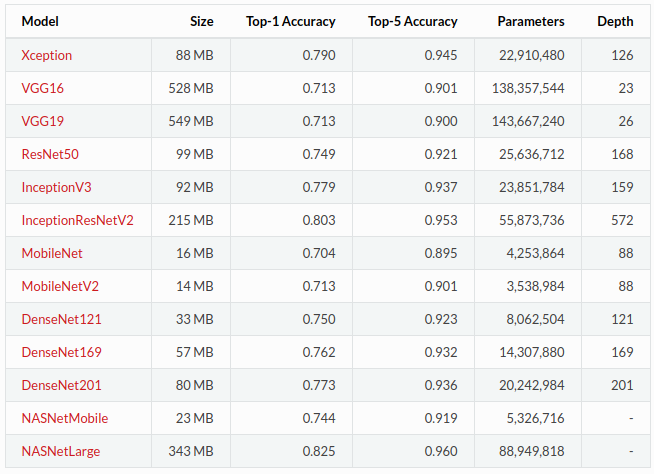
\includegraphics[width=0.70\textwidth]{trancomp.png}
\end{figure}




\subsection{Hyper Parameter Optimization}

So far we introduced different parameters. We can classify them into two categories; learnable parameters an hyper-parameters. In the first category we have weights and biases which we update in gradient decent. Hyper-paramters are the ones we set prior to training. Number of layers or neurons, learning rate, momentum, number of epochs, weight decay, batch size and other problem-based parameters are considered as hyperparamters. Finding the optimal values for those parameters can be a very challenging task and there is a huge research efforts in this area. Actually one can define an \textit{hyper-parameter space} and search for the optimal values which can provide an efficient and accurate way of building an architecture. However when we consider the number of parameters and the size of the training set in practical applications, it is obvious that this effort can require a substantial computing resources, such as paralelization on multiple GPUs and large clusters.
\section{An Image Classification Problem}

In this section, we will apply the techniques we introduced above for an image classification problem. We will work on the Intel Image Classification problem \cite{intel}. Data contains around 25k images of size $150x150$ distributed under 6 categories; \\

'building' : 0, 'forest': 1, 'glacier' : 2, 'mountain' : 3, 'sea' : 4, 'street' : 5 \\

There are around 14k images in training set, 3k in validation set and 7k for prediction. We will use one of the most well-known Python machine learning library \textit{Pytorch}. In this report, we design two different architectures.In practical applications, it is very common to start with a pretrained model. So In the first one, we implement a transfer learning with VGG16 \cite{vgg16}.We achieved \%92.5 test accuracy and \%94.1 training accuracy and reported several other results. We also design a custom convolutional neural network and try to fine tune using the techniques introduced above. We obtained \%86 testing accuracy here at the time we finish the report but we will spend more time on it in the future.


%\subsection{General Strategy}

In order to create a neural network in Pytorch, we use \textit{torch.nn} package which contains necessary building blocks to build a network. Within nn package, we have \textit{nn.Modules} class which is the base class for all of the other neural net modules. So the core idea in neural network programming in pytorch is to build the architecture on the top of \textit{nn.Modules},i.e, we define the model as a subclass of \textit{nn.Modules}. Once we we create the architecture, we should define a forward pass method. To do so we must overwrite \textit{nn.Modules}'s \textit{forward()} method. To do so, we use some functionalities (cost functions, activation functions, dropout, pooling, calculating the gradients etc) provided by \textit{nn.Functional} package. Once we have the gradients, we can update the weights and biases or other learnable parameters using \textit{nn.Optim} package. 

Once we have the architecture with the necessary components, we can develop a strategy for hyper parameter estimation. There is no single best way to do it but our strategy is to create a cartesian product of some of the learnable parameters in outermost loop and train the model over a single element of this product space. We can call this product as hyperspace and define as
\begin{equation}
\label{eq:hspace}
H_{1}xH_{2}x..H_{n} = \{(h_{1},h_{2},..h_{n}): h_{1} \in \{\text{learning rates}\}, h_{2}\in \{\text{batch sizes}\}, .. \}
\end{equation}
We will then enter the training loop, monitor the outcomes such as loss, accuracy and pass them to the \textit{Tensorboard} environment \cite{tb} which is a great tool to visualize the outcomes for post processing. In the same loop, we will also write the outcomes in a csv file using python data analysis library \textit{pandas} \cite{pandas} for further processing. Note that even few elements in each set in (\ref{eq:hspace}) results a large product space. For example three hyper parameter sets each having 4 elements yield a product space with 64 elements. Thus we will use a small epoch value in the training loop. 

\textit{Personal note: I started to learn neural network when I was a PhD student in Mathematics and Statistics at Texas Tech University and typed this report in a couple of weeks in the scope of an individual study. That was my first exposure to neural networks. Grid search is always the first destination for new learners to perform hyperparameter optimization. However, the reader of this report should note that it \textbf{the worst} and the most expensive strategy as well. This is an active research topic. The better practice would be to integrate an hyperarameter optimization library endowed with the state-of-the-art methods into your framework. The project above can be found in my github at \cite{intel1} without the use of such library. However, I studied one of the most popular hyperarameter tuning frameworks \textit{Optuna} \cite{optuna} and integrated it into a different image classification \cite{syms} and also image segmentation projects \cite{segment}
I would like to keep the discussion above in the current text for personal reasons}.






%\section{Some Theoretical Aspects }
%	\subsection{Universal Approximation Theorem}
%	\subsection{Converge of Gradient Decent}
%
%%In this section, we will briefly describe the mathematical aspects of neural network architectures. Let $\bm{h}$ and 
%%$\bm{d_{m}}$ denote the depth and the width of the architecture and $\bm{n}$ be the number of input neurons or input dimension.  
%%
%% In the next section, we will formally define the the mathematical relationship between the layers of a network but we briefly state here for the sake of completeness. For a single neuron, say   
%Look at the recommendation paper!!
%
%
%
%

\bibliographystyle{unsrt}
\bibliography{report}



\end{document}
